\documentclass[../main.tex]{subfiles}
%\usepackage[T1]{fontenc}
%\usepackage[utf8]{inputenc}
%\usepackage{geometry}   
%\usepackage{float}
%\usepackage[section]{placeins}
%\usepackage{amsmath}
%\usepackage{amssymb}
%\usepackage{amsfonts}
%\usepackage[colorlinks=true, allcolors=blue]{hyperref}
%\usepackage{mathtools}
%\usepackage[switch, mathlines]{lineno}
%\usepackage[usenames,dvipsnames]{xcolor} 
%\usepackage[normalem]{ulem}
%\usepackage[capitalise,nameinlink]{cleveref}
%\usepackage{enumitem}
%\usepackage{csquotes}
%\usepackage{xspace}
%\usepackage{multirow}
%\usepackage{tabularx}
%\usepackage{color, colortbl}
%\usepackage[colorinlistoftodos]{todonotes}
%\usepackage{graphicx}
%
%% for writing code blocks 
%\usepackage{listings}
%%\usepackage{color}
%\usepackage{caption}
%\usepackage{subcaption}
%\definecolor{orange}{rgb}{1,0.5,0}
%\definecolor{darkorange}{rgb}{0.69,0.33,0.13}
%\definecolor{fidcol}{rgb}{0.7,0,0}
%\definecolor{mkcol}{rgb}{0.5,0,0.5}
%\definecolor{mmcol}{rgb}{0.7,0.17,0.31}
%\definecolor{dscol}{rgb}{0.6,0.1,0.2}
%\definecolor{mccol}{rgb}{0.2,0.4,0.6}
%\definecolor{darkgreen}{rgb}{0.05,0.5,0.06}
%\definecolor{carnelian}{rgb}{0.7, 0.11, 0.11}
%\definecolor{dkgreen}{rgb}{0,0.6,0}
%\definecolor{mauve}{rgb}{0.58,0,0.82}
%\definecolor{gray}{gray}{0.9}
%\definecolor{cyan}{rgb}{0.88,1,1}
%
%\newcommand*{\Euclid}{\textit{Euclid}\xspace}
%\newcommand*{\Planck}{\textit{Planck}\xspace}
%\newcommand*{\rd}{\mathrm{d}}
%\newcommand*{\rD}{\mathrm{D}}
%\newcommand*{\marktodo}{{\color{mmcol} ::TODO::}\xspace}
%\newcommand*{\halofit}{\texttt{HALOFIT}\xspace}
%\newcommand*{\hmcode}{\texttt{HMCODE}\xspace}
%\newcommand*{\montepython}{\texttt{MP}\xspace}
%\newcommand*{\cosmicfish}{\texttt{CF}\xspace}
%\newcommand*{\class}{{\tt CLASS}\xspace}
%\newcommand*{\camb}{{\tt CAMB}\xspace}
%\newcommand*{\montefisher}{\texttt{MP:Fisher}\xspace}
%
%\newcommand*{\neff}{N_\mathrm{eff}}

\begin{document}
\chapter{Results}
In this chapter, we present our forecast results for neutrino parameters and dark energy. We remind ourselves that the validation runs were not actual forecasts. For them, we used extra optimistic settings to be able to find good agreement for the FI matrixes. For the forecast, we will switch to more realistic and conservative settings. Compared to our validation runs there are multiple differences in our parameters. Firstly the neutrino mass $m_\nu$ is no longer condensed into one massive neutrino but evenly split between three neutrino species. To differentiate this quantity from the neutrino mass from the last chapter we will call it $\sum m_\nu$. This is done by setting the number of degenerate non-cold dark matter particles '${\tt deg_ncdm=3}$'.\\
Because of this we also change our definition of $N_\mathrm{eff}$. Before it could have been understood as a change in the temperature of the massless neutrinos and could vary freely to higher and lower values. Now all neutrinos have the same temperature of \begin{equation}
    T_{\nu} = T_\mathrm{CMB}\,\left(\frac{3.044}{3}\right)^{1/4}\,\left(\frac{11}{4}\right)^{1/3}.
\end{equation}
This parameter now just parametrises any additional massless relic particle. Typical models only predict additional species that contribute positively to $N_\mathrm{eff}$. From this, we define a new parameter $\Delta N_\mathrm{eff}$. This parameter is essentially equivalent to the parameter $N_\mathrm{ur}$ inside of \class.\\
Our next change is, that we vary the parameters $\sigma_v$ and $\sigma_p$ that govern the nonlinear corrections of the spectroscopic probe. In order to be more conservative we also stick to the pessimistic settings of the probes. We will also vary all 9 cosmological parameters for our MCMC.\\
For $\sum m_\nu$ and $\Delta N_\mathrm{eff}$ we chose prior edges with a theoretical prior at 0 as a lower bound and an upper bound high enough to not change our results. The dark energy parameters have a bit tighter prior edges to not probe unphysical regions of the parameter space. These parameters are an approximation to a wider set of theories where dark energy has an equation of state that is slowly varying. When the posterior hits the prior edges for the dark energy parameters we will consider them as unconstrained. For the other cosmological and nuisance parameters we have chosen arbitrary priors that will not be reached but speed up convergence.\\
A summary of our cosmological parameters, their fiducial and their prior edges can be seen in the table \ref{tab:fiducial_forecast}. 
\begin{table}[t]
    \renewcommand{\arraystretch}{1.2}
        \caption{Settings for the final forecast MCMCs. The fiducial values of the Nuisance parameters have been listed in the section for the respective probes. }
        \centering
        \begin{tabular}{ccccccccc}
        \hline
        \rowcolor{cyan} \multicolumn{9} {c}{{\bf{Varied parameters}}}\\ 
     \multicolumn{1}{c}{$\Omega_{\rm m}$} & \multicolumn{1}{c}{$100\times\Omega_{\rm b}$} & \multicolumn{1}{c}{$h$} & \multicolumn{1}{c}{$n_{\rm s}$} & \multicolumn{1}{c}{$\sigma_{8}$} & \multicolumn{1}{c}{$\sum m_\nu$(meV)} & \multicolumn{1}{c}{$\Delta \neff$} & \multicolumn{1}{c}{$w_0$} & \multicolumn{1}{c}{$w_a$} \\
      \hline
      \rowcolor{gray} \multicolumn{9} {c}{{{Fiducal Value}}}\\
            0.314571 & 4.92 & $0.6737$ & $0.9661$ & $0.81$ & $60$ & $0 $& $0$ & $-1$ \\
            \hline
            \rowcolor{gray} \multicolumn{9} {c}{{{Prior Edges}}}\\
            $[0.005,1]$&$[0.5,100]$&$[0.1,1.5]$&$[0.8,1.2]$&$[0.7,0.9]$&$[0,1000]$&$[0,5]$&$[-1.5,-0.5]$&$[-1,1]$
        \end{tabular}
        %}
        \label{tab:fiducial_forecast}
    \end{table}
    \begin{figure}
        \centering
        \caption{One and two-dimensional marginalized posteriors for the different \Euclid probes. We depict the 68\% and 95\% confidence intervals for the cosmological parameters of the full nine-parameter model. We depict the photometric probe in purple, the spectroscopic probe in cream and the combined probe in red.}
        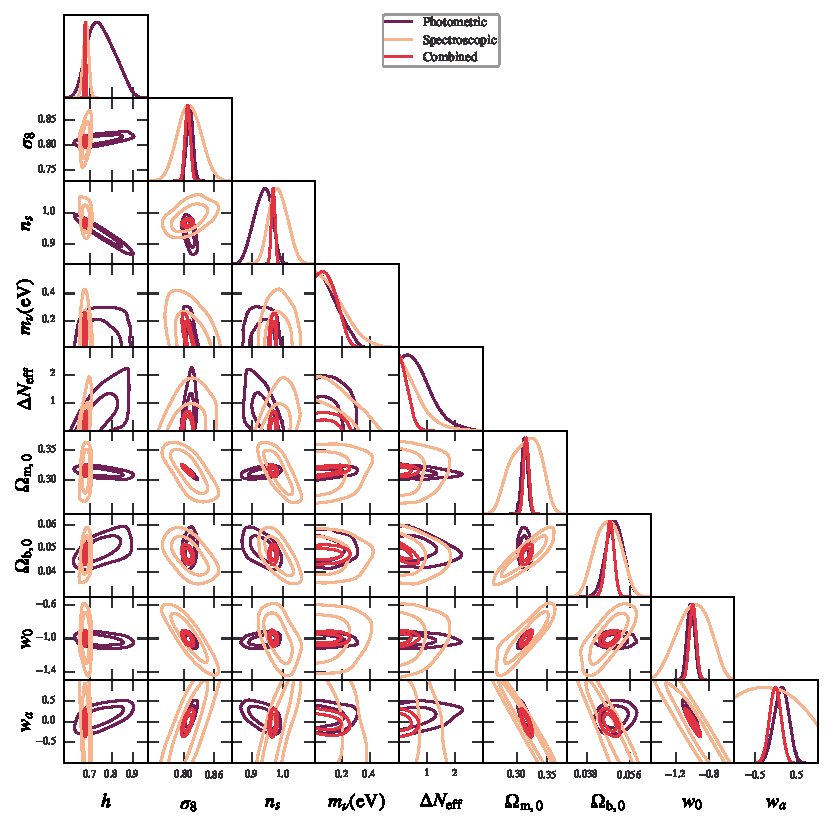
\includegraphics[width=1.0\linewidth]{../plots/results_trianle.pdf}
        \label{fig:results_trianle}
    \end{figure}
    The results can be seen in figure \ref{fig:results_trianle}. We see that the photometric and spectroscopic probes are sensitive to different cosmological parameters. The spectroscopic probe dominates the sensitivity for $\Delta \neff$ and $h$. These are the parameters that mainly affect the BAO. Since the spectroscopic probe is sensitive to that region, it measures these well. The spectroscopic probe is nearly insensitive to the amplitude of the power spectrum as it is multiplied by the galaxy biases. To break this, the spectroscopic probe needs the RSD where the clustering parameter $f\,\sigma_8$ enters. We also see that it alone is not able to constrain the time-dependent dark energy equation of state parameter $w_a$. This parameter controls only slightly the time evolution of the amplitude of the matter power spectrum. Its sensitivity to the baryon density parameter $\Omega_b$ is greatly reduced by varying $\sigma_v$. This is due to the effect of $\Omega_b$ in shifting the phase of the BAO can also be mimicked by varying $\sigma_v$.\\
    The photometric probe is very sensitive to the amplitude of the power spectrum and dominates the dark energy parameters, the neutrino mass, the density parameter of total matter, and the variance of the matter perturbations. Its sensitivity to $\Omega_b$ comes also from the BAO that leaves a small impact on the actual $C_l$. Since the scale of the BAO is fixed at around $5\cdot10^{-2} \mathrm{Mpc}^{-1}$ the imprint shows up at different multipoles $\ell$ for different redshift bins. This leaves a very clear signature of $\Omega_b$. It loses its sensitivity to $h$ and $\Delta \neff$ for the same reason. The actual scale of the BAO is washed out by the integration over $z$ for each bin. Essentially this makes the photometric probe lose its sensitivity to scales.\\
    In that sense, both probes are very complimentary to each other. In the figure, one can see how the correlation directions of the different probes are often perpendicular to one another breaking correlation directions and drastically improving the constraints on $h$, $n_s$, and $\Delta \neff$.\\
    Nevertheless, judging from this forecast, Euclid alone will not be able to detect the neutrino mass. This is why in our final forecasting results in tabel we can only give a 95\% confidence interval. It should be noted that by adding CMB data to our forecast, we can achieve a measurement of the neutrino mass on the 68\% confidence level for this nine-parameter model. If we go to a smaller model with only $\Lambda$CDM+$m_\nu$ we can even achieve a 99\% confidence detection. We will not discuss these results further in this work as we have not discussed the CMB as an additional probe.\\
    The marginalized errors are found in the table \ref{tab:results}. The constraints of \Euclid for the cosmological parameters are tighter than for \Planck. \Planck does not have the constraining power to constrain dark energy and neutrinos at the same time. Nevertheless, we can compare the constraints on the cited sensitivities of the submodels. This is beacuse the parameters $w_0+w_a$ are not to strongly correlated with the other two parameters  in our case. This makes it so that the constraints stay similar, because we are not opening up correlation directions. This means that we expect similar errors for the parameters if we have run the smaller models. In an analysis of the $w_0w_a$CDM \Planck + BAO + Supernovae gives constraints on the dark energy parameters \begin{align*}
        w_0 = -0.957 \pm 0.08 \quad \text{and}\quad w_a = -0.29 \pm 0.3
    \end{align*}
    This means that we can constrain these parameters better with the bigger model. The main part of the constraints of \Planck to these parameters are from contributions in additional late integrated Sachs-Wolf effect. This essentially comes from the fact that during dark energy domination, the metric perturbations start to decay adding some additional terms to the low multipole $C_\ell$ of CMB. With \Euclid we can see the same redshift-dependent reduction of the amplitude on all scales due to its tomographic nature. This is strongly constraining for these dark energy parameters.\\
    The parameters $\sum m_\nu$ and $\Delta N_\mathrm{eff}$ are constrained by \Planck+BAO+lensing to 
    \begin{equation}
        \sum m_\nu < 0.12 \quad \text{and}\quad \Delta N_\mathrm{eff} < 0.34.
    \end{equation}
    These are both tighter than in our \Euclid forecast. The main sensitivity to these parameters comes from their background effects shifting the angular scale of recombination and the redshift of equality. Both of these parameters are very tightly constrained by the CMB measurements.\\
    As both experiments measure probes that are very complimentary to one another as well as having additional Information in their cross-correlation, we believe that a combined analysis will bring us a new milestone in precision cosmology.
    \begin{table}[!h]
        \renewcommand{\arraystretch}{1.2}
          \centering
        \caption{Forecast 68\% confidence levels for the different \Euclid probes and the combined probe. For the parameters $\sum m_\nu$ and $\Delta \neff$ we only state the 95\% upper limit as they are bound from below by their theoretical prior. The spectroscopic probe alone was not able to constrain $w_a$ within our prior edges.}
          \resizebox{\textwidth}{!}{
        \begin{tabular}{l|ccccccc|cc}
\hline
    \rowcolor{cyan}    \multicolumn{10} {c}{{\textbf{Forecast Results}}} \\
    \multicolumn{1}{c}{}&\multicolumn{1}{c}{$\Omega_{\rm m}$} & \multicolumn{1}{c}{$100\times\Omega_{\rm b}$} & \multicolumn{1}{c}{$h$} & \multicolumn{1}{c}{$n_{\rm s}$} & \multicolumn{1}{c}{$\sigma_{8}$}  & \multicolumn{1}{c}{$w_0$} & \multicolumn{1}{c}{$w_a$} &\multicolumn{1}{c}{$\sum m_\nu$(meV)} & \multicolumn{1}{c}{$\Delta \neff$}\\
    \hline
    \rowcolor{gray}Probe&\multicolumn{7}{|c}{68\% Sensitivity}&\multicolumn{2}{|c}{95\% confidence limit}\\
Photometric	&$0.0049$	&$0.38$	&$0.065$	&$0.029$	&$0.0065$	    	&$0.05$	&$0.18$&$<260.$	&$<1.70$	\\ 
Spectroscopic	&$0.0258$	&$0.56$	&$0.013$	&$0.031$	&$0.024$		&$0.20$	&$ -$&$<350.$	&$<1.50$	\\ 
Combined	&$0.0043$	&$0.18$	&$0.0030$	&$0.0060$	&$0.0054$		&$0.04$	&$0.14$	&$<220.$	&$<0.57$\\ 
\end{tabular}

}

\label{tab:results}
\end{table}
\end{document}
